\documentclass[compress]{beamer}
\usepackage{ifthen,verbatim}

\newcommand{\isnote}{}
\xdefinecolor{lightyellow}{rgb}{1.,1.,0.25}
\xdefinecolor{darkblue}{rgb}{0.1,0.1,0.7}

%% Uncomment this to get annotations
%% \def\notes{\addtocounter{page}{-1}
%%            \renewcommand{\isnote}{*}
%% 	   \beamertemplateshadingbackground{lightyellow}{white}
%%            \begin{frame}
%%            \frametitle{Notes for the previous page (page \insertpagenumber)}
%%            \itemize}
%% \def\endnotes{\enditemize
%% 	      \end{frame}
%%               \beamertemplateshadingbackground{white}{white}
%%               \renewcommand{\isnote}{}}

%% Uncomment this to not get annotations
\def\notes{\comment}
\def\endnotes{\endcomment}

\setbeamertemplate{navigation symbols}{}
\setbeamertemplate{headline}{\mbox{ } \hfill
\begin{minipage}{5.5 cm}
\vspace{-0.75 cm} \small
\end{minipage} \hfill
\begin{minipage}{4.5 cm}
\vspace{-0.75 cm} \small
\begin{flushright}
\ifthenelse{\equal{\insertpagenumber}{1}}{}{Jim Pivarski \hspace{0.2 cm} \insertpagenumber\isnote/\pageref{numpages}}
\end{flushright}
\end{minipage}\mbox{\hspace{0.2 cm}}\includegraphics[height=1 cm]{../cmslogo} \hspace{0.1 cm} \includegraphics[height=1 cm]{../tamulogo} \hspace{0.01 cm} \vspace{-1.05 cm}}

\begin{document}
\begin{frame}
\vfill
\begin{center}
\textcolor{darkblue}{\Large Beam-halo Alignment with Constants}

\vfill
\begin{columns}
\column{0.3\linewidth}
\begin{center}
\large
\textcolor{darkblue}{\it Jim Pivarski}

Aysen Tatarinov

Vadim Khotilovich

Alexei Safonov
\end{center}
\end{columns}

\begin{columns}
\column{0.3\linewidth}
\begin{center}
\scriptsize
{\it Texas A\&M University}
\end{center}
\end{columns}

\vfill
12 May, 2010

\end{center}
\end{frame}

%% \begin{notes}
%% \item This is the annotated version of my talk.
%% \item If you want the version that I am presenting, download the one
%% labeled ``slides'' on Indico (or just ignore these yellow pages).
%% \item The annotated version is provided for extra detail and a written
%% record of comments that I intend to make orally.
%% \item Yellow notes refer to the content on the {\it previous} page.
%% \item All other slides are identical for the two versions.
%% \end{notes}

\small

%% \begin{frame}
%% \frametitle{Outline}
%% \begin{itemize}\setlength{\itemsep}{0.75 cm}
%% \item 
%% \end{itemize}
%% %% \hspace{-0.83 cm} \textcolor{darkblue}{\Large Outline2}
%% \end{frame}

%% \section*{First section}
%% \begin{frame}
%% \begin{center}
%% \Huge \textcolor{blue}{First section}
%% \end{center}
%% \end{frame}

\begin{frame}
\frametitle{Ring-radius corrections}

\begin{itemize}
\item Last week, I showed that ring-radius corrections estimated from
  disk-bending improve track-based closure by a factor of 2

\item If we assume that the remaining non-closure is due to wrong
  ring-radii, we can apply it as a track-based correction
\begin{itemize}
\item strong assumption that the internal CSC geometry is correct
\item closure was zero in 2008 $\vec{B}=0$ data
\end{itemize}

\item Size of these corrections (after all others have been applied)
  have an interesting pattern:
\begin{center}
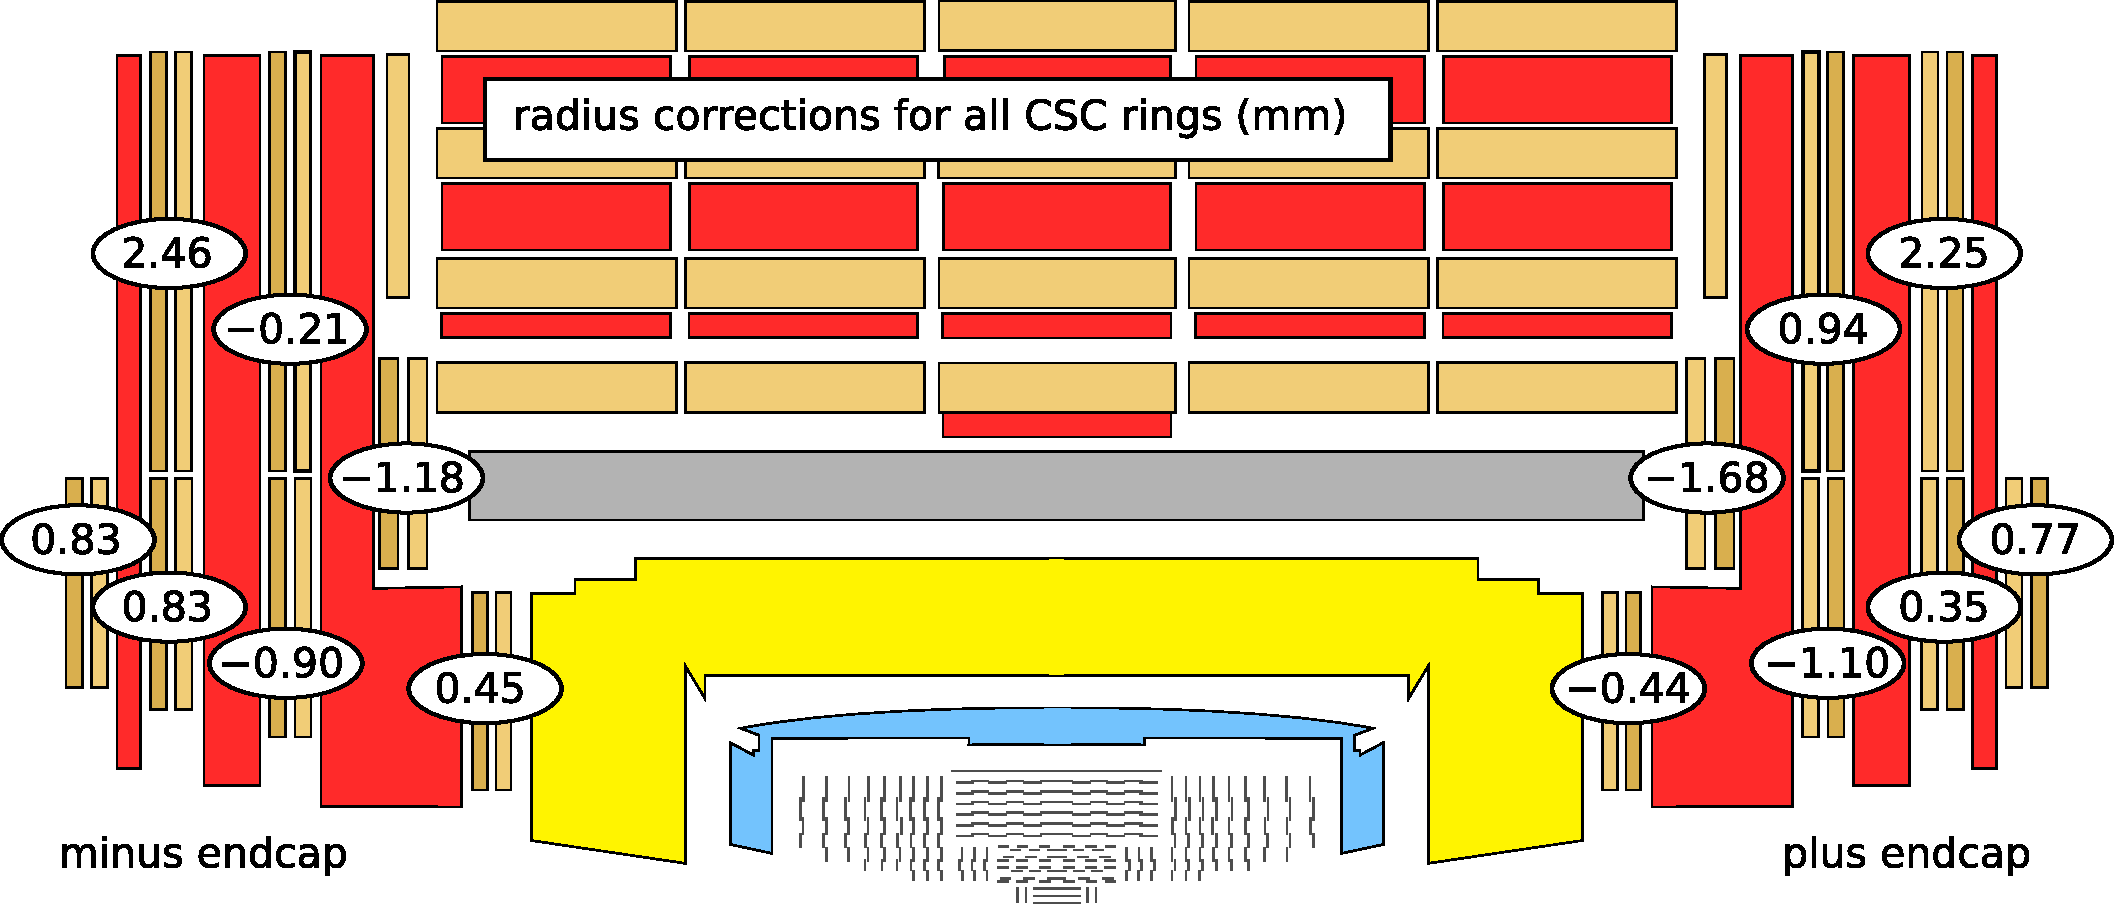
\includegraphics[width=0.8\linewidth]{radial_corrections.pdf}
\end{center}
\end{itemize}
\end{frame}

\begin{frame}
\frametitle{New constants ({\it nearly} final)}

\begin{itemize}
\item Assuming the new ring-radii is a prerequisite for $r\phi$ alignment

\item New constants, assuming the new ring-radii

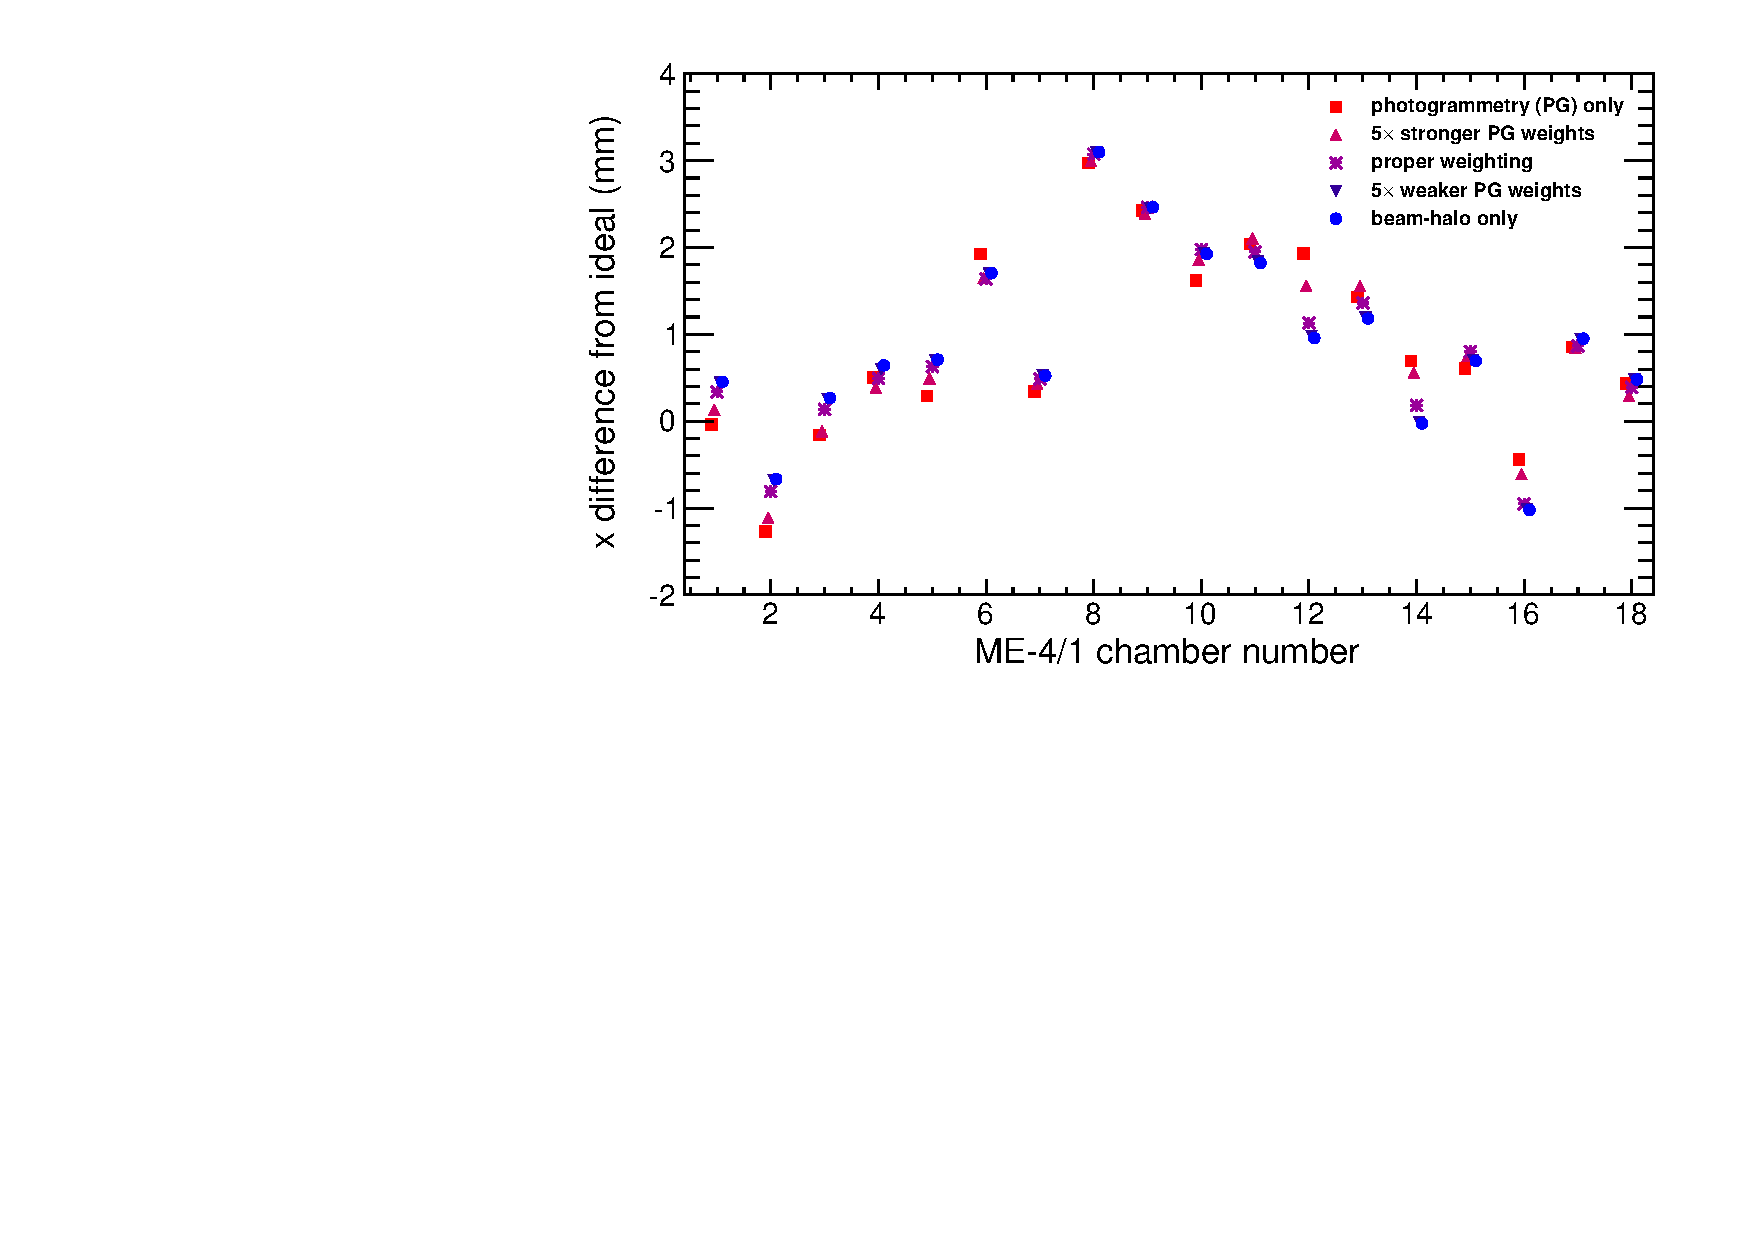
\includegraphics[width=\linewidth]{dependence_on_weights_41.pdf}

\item Pure PG is not very far from pure beam-halo, but now we can
  align them in a combined fit (demonstrated by varying weights)
\end{itemize}
\end{frame}

\begin{frame}
\frametitle{New constants ({\it nearly} final)}

\begin{itemize}
\item Another example: this ring has incomplete PG
\item Pure PG has no information about this chamber (set to ideal),
  but even strongly-weighted PG yields a reasonable value for the missing
  chamber because it is ``filled in'' by beam-halo data
\end{itemize}

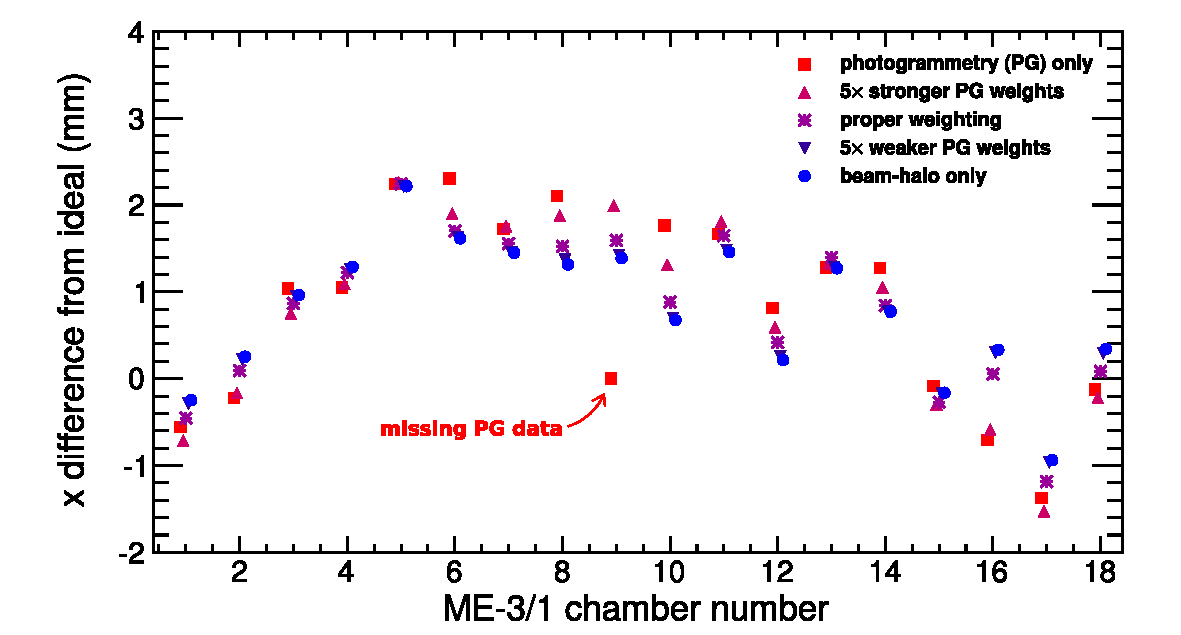
\includegraphics[width=\linewidth]{dependence_on_weights_31.pdf}
\end{frame}

\begin{frame}
\frametitle{New constants ({\it nearly} final)}

\begin{itemize}
\item This ring has incomplete beam-halo; system of equations cannot
  be solved without external information
\item Even weakly-weighted PG yields a reasonable value for the
  missing overlap
\end{itemize}

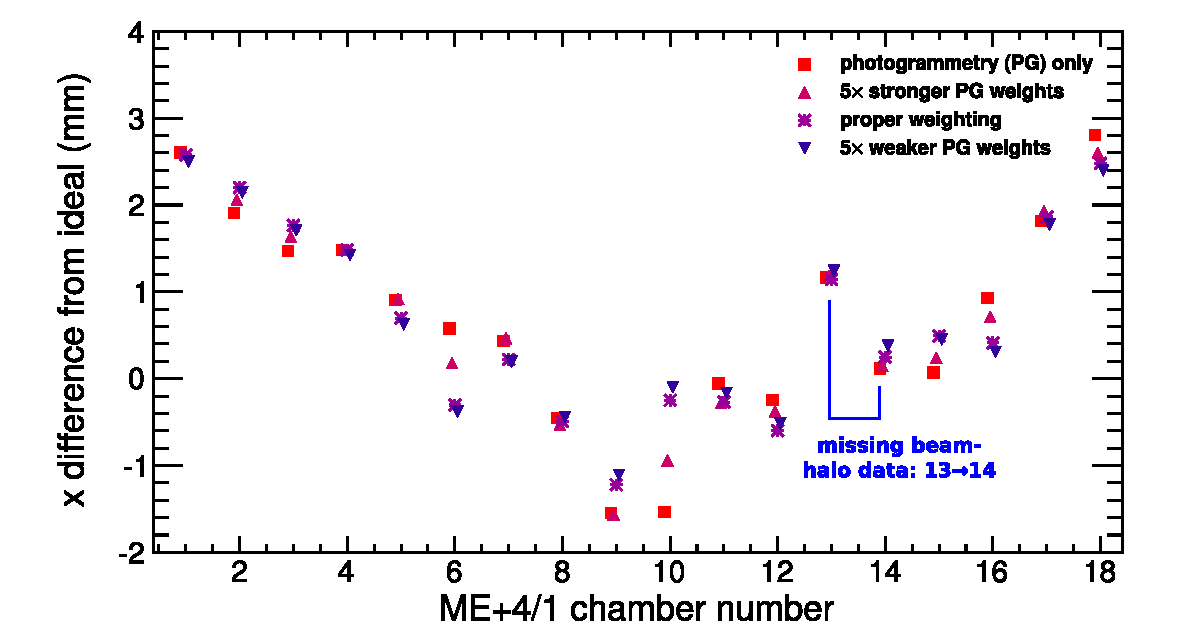
\includegraphics[width=\linewidth]{dependence_on_weights_p41.pdf}
\end{frame}

\begin{frame}
\frametitle{New constants ({\it nearly} final)}

\begin{itemize}
\item An outer ring (low beam-halo statistics) with several missing
  chambers in a row: the relative positions of these are entirely
  determined by PG
\end{itemize}

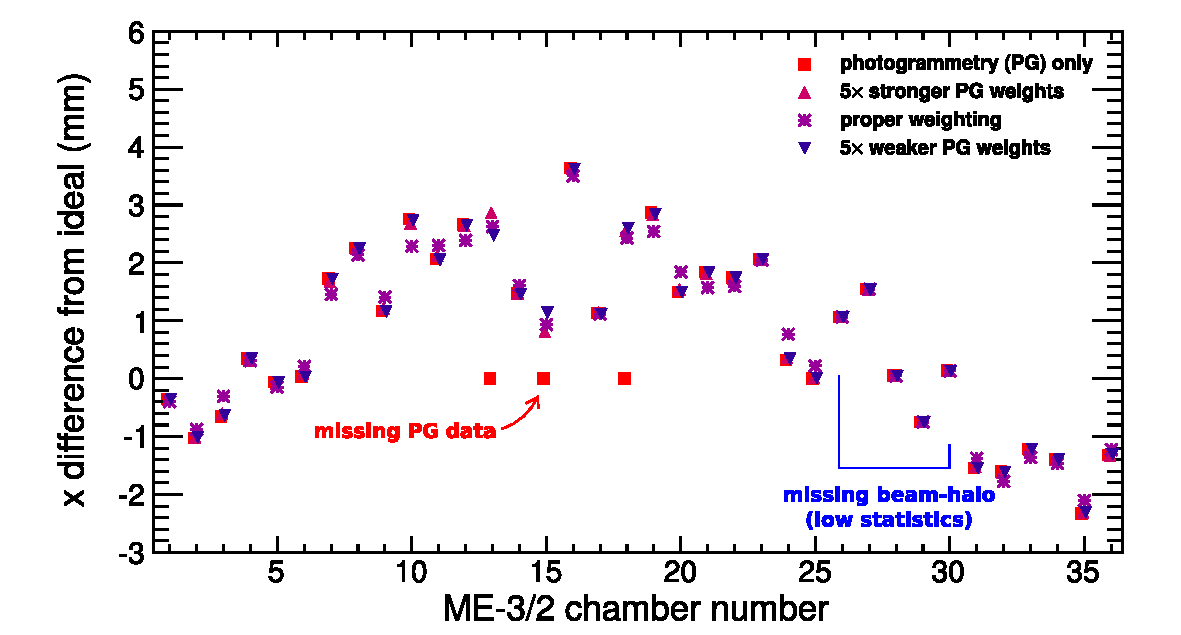
\includegraphics[width=\linewidth]{dependence_on_weights_32.pdf}
\end{frame}

\begin{frame}
\frametitle{New constants ({\it nearly} final)}

\begin{itemize}
\item Also works for $\phi_z$ rotation angle

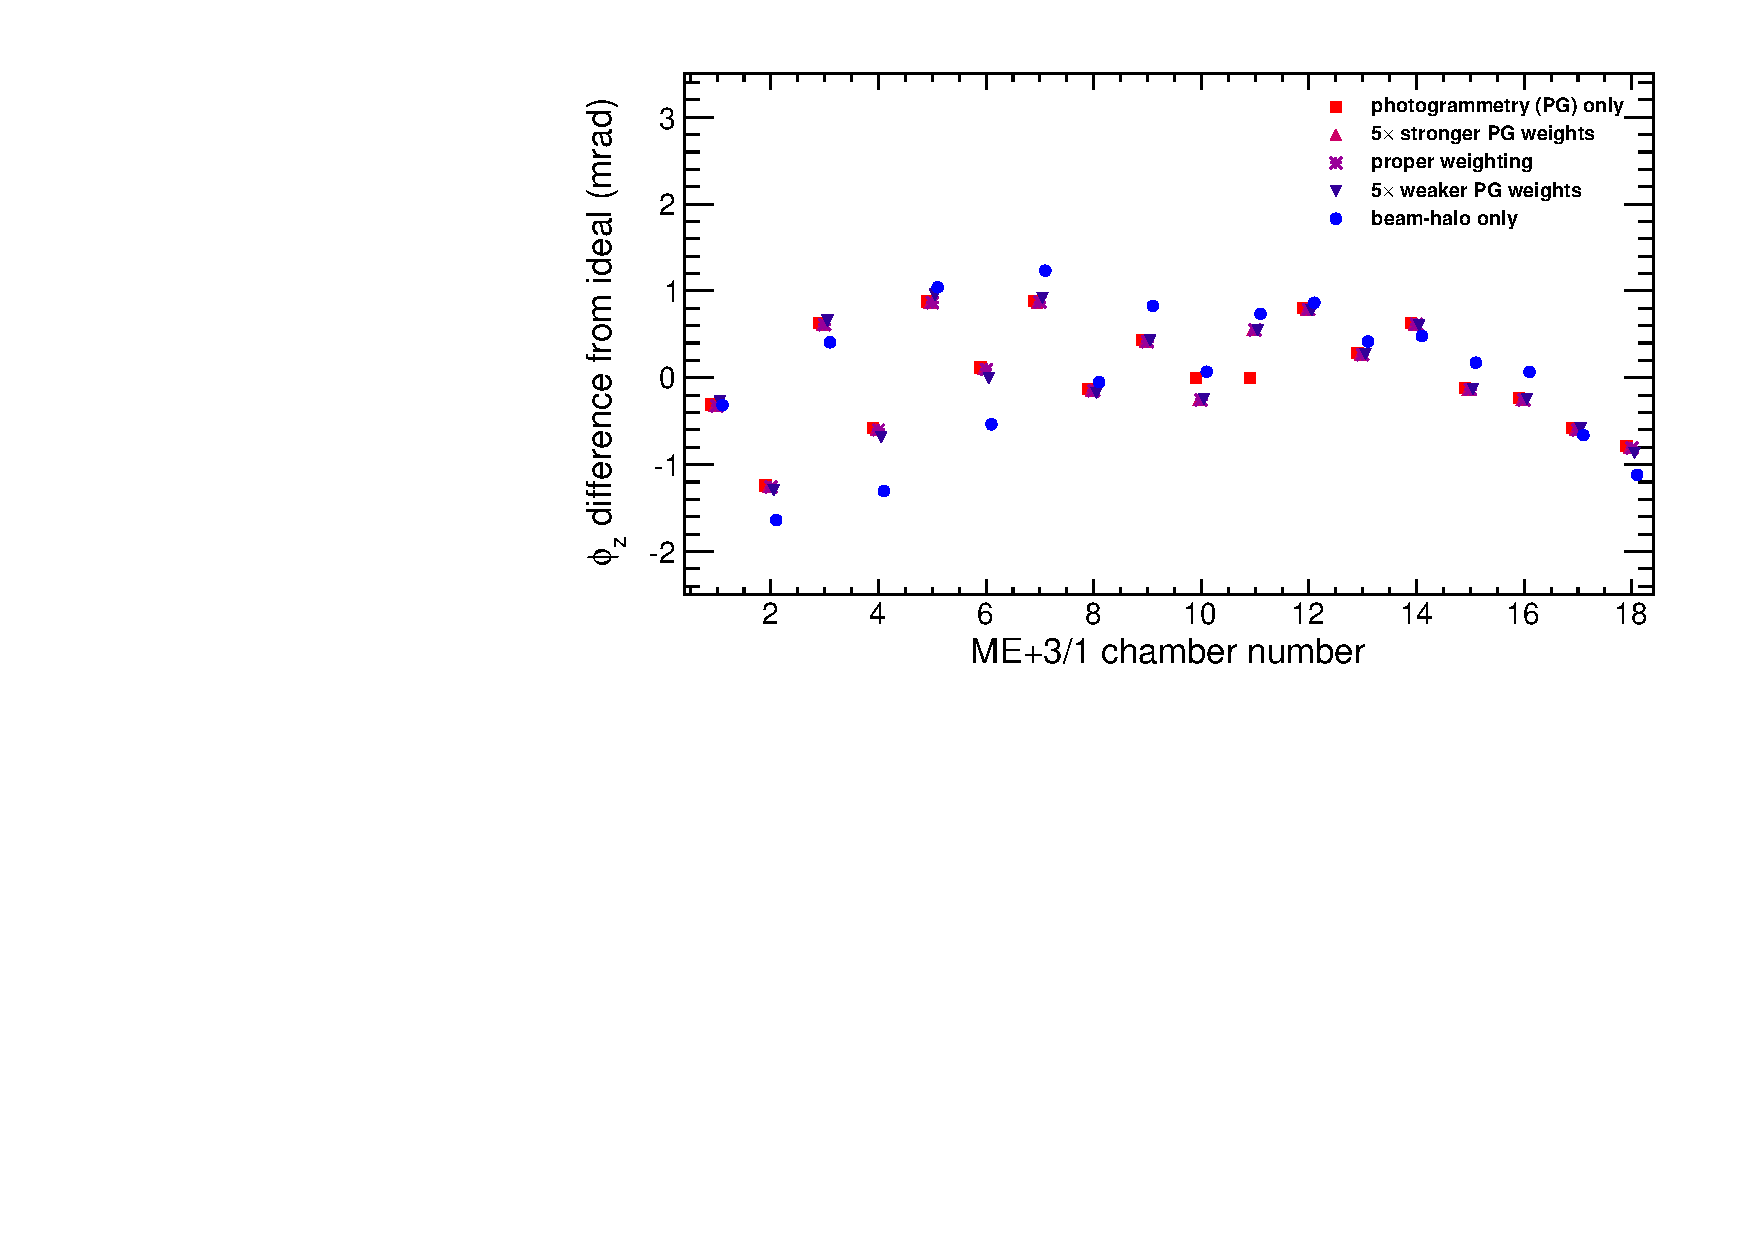
\includegraphics[width=\linewidth]{dependence_on_weights_p31phiz.pdf}

\item Two alignment parameters, $r\phi$ and $\phi_z$, in addition to ring radii
\begin{itemize}
\item third possible parameter, $\phi_y$, is imprecise when measured
  with beam-halo (ideal geometry is more accurate, so leave as ideal)
\end{itemize}
\end{itemize}
\end{frame}

\begin{frame}
\frametitle{New constants ({\it nearly} final)}

\begin{itemize}
\item ME1/1 is a special case: PG constraints are not compatible with
  beam-halo data, so they could not be combined

\href{https://hypernews.cern.ch/HyperNews/CMS/get/muon-alignment/512.html?inline=-1}{\tt \tiny https://hypernews.cern.ch/HyperNews/CMS/get/muon-alignment/512.html?inline=-1}

\item Alignment graph is not fully connected, not a complete solution
\end{itemize}

\begin{columns}
\column{0.6\linewidth}
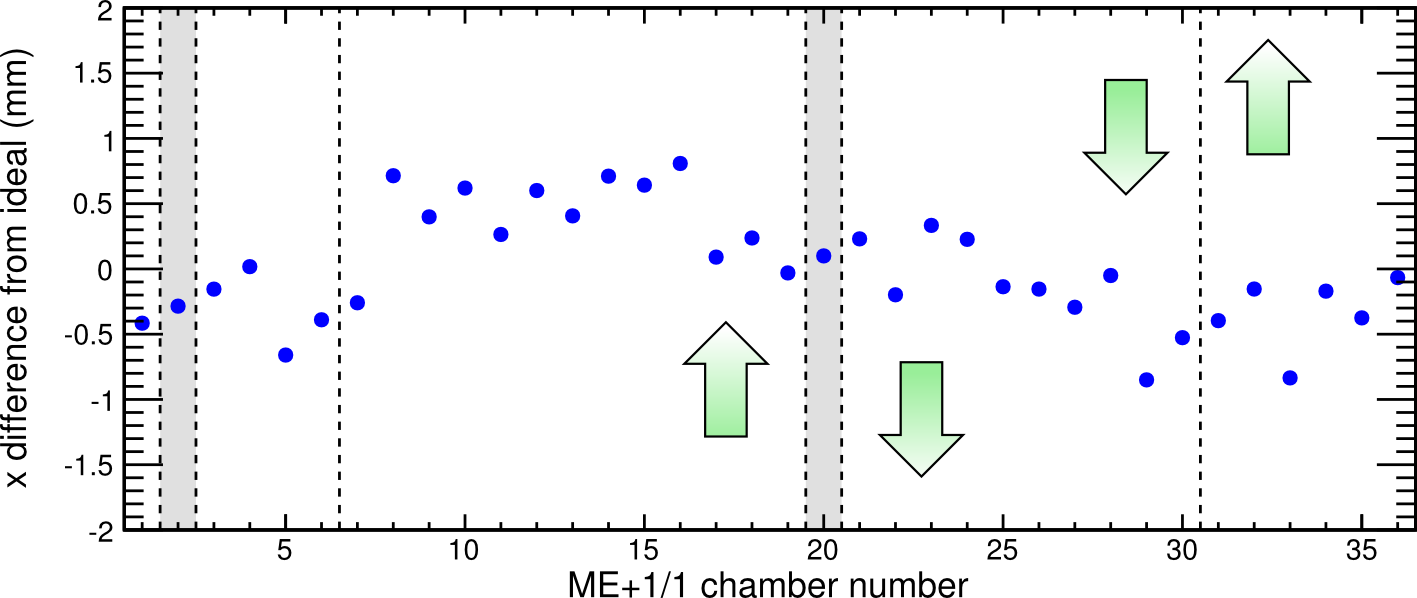
\includegraphics[width=\linewidth]{dependence_on_weights_p11.png}

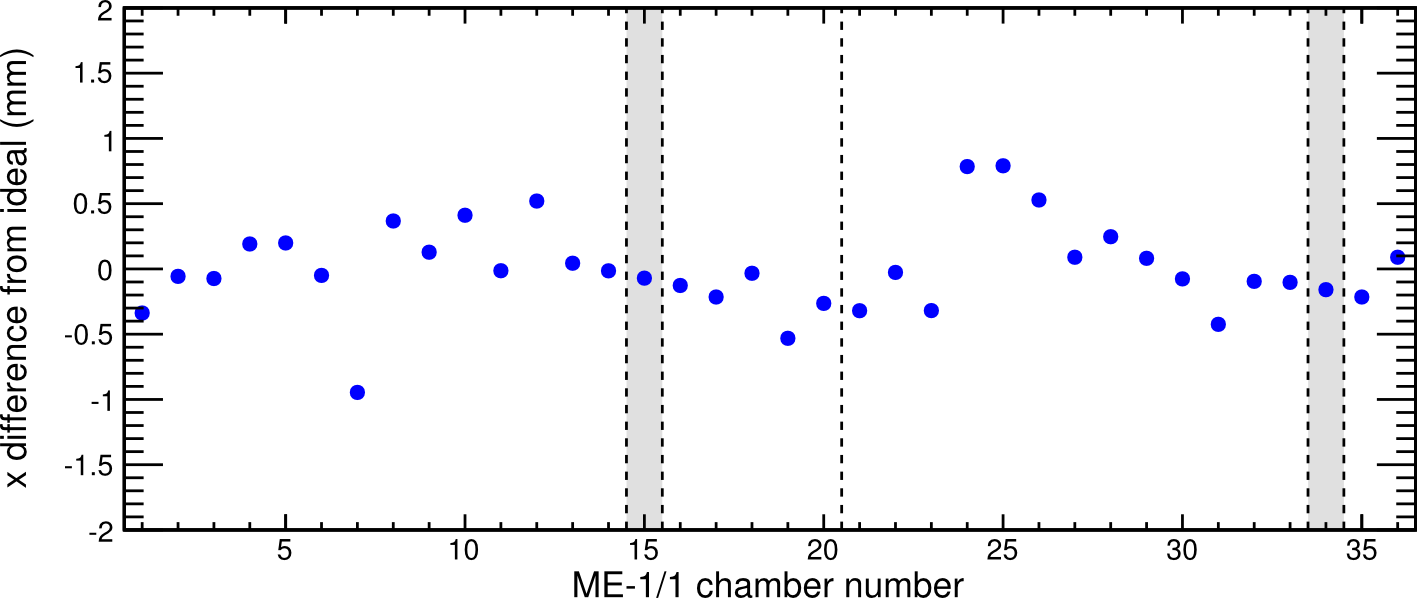
\includegraphics[width=\linewidth]{dependence_on_weights_m11.png}

\column{0.45\linewidth}
\begin{itemize}
\item Dashed lines indicate missing connections

\item We can align the disconnected sections, but these sections will
  later need to be positioned relative to the tracker using
  globalMuons

\item Interestingly, ME1/1 geometry is nearly ideal (more so than other rings)
\end{itemize}
\end{columns}
\end{frame}

\begin{frame}
\frametitle{Compatibility of PG and BH}

\begin{columns}
\column{0.6\linewidth}
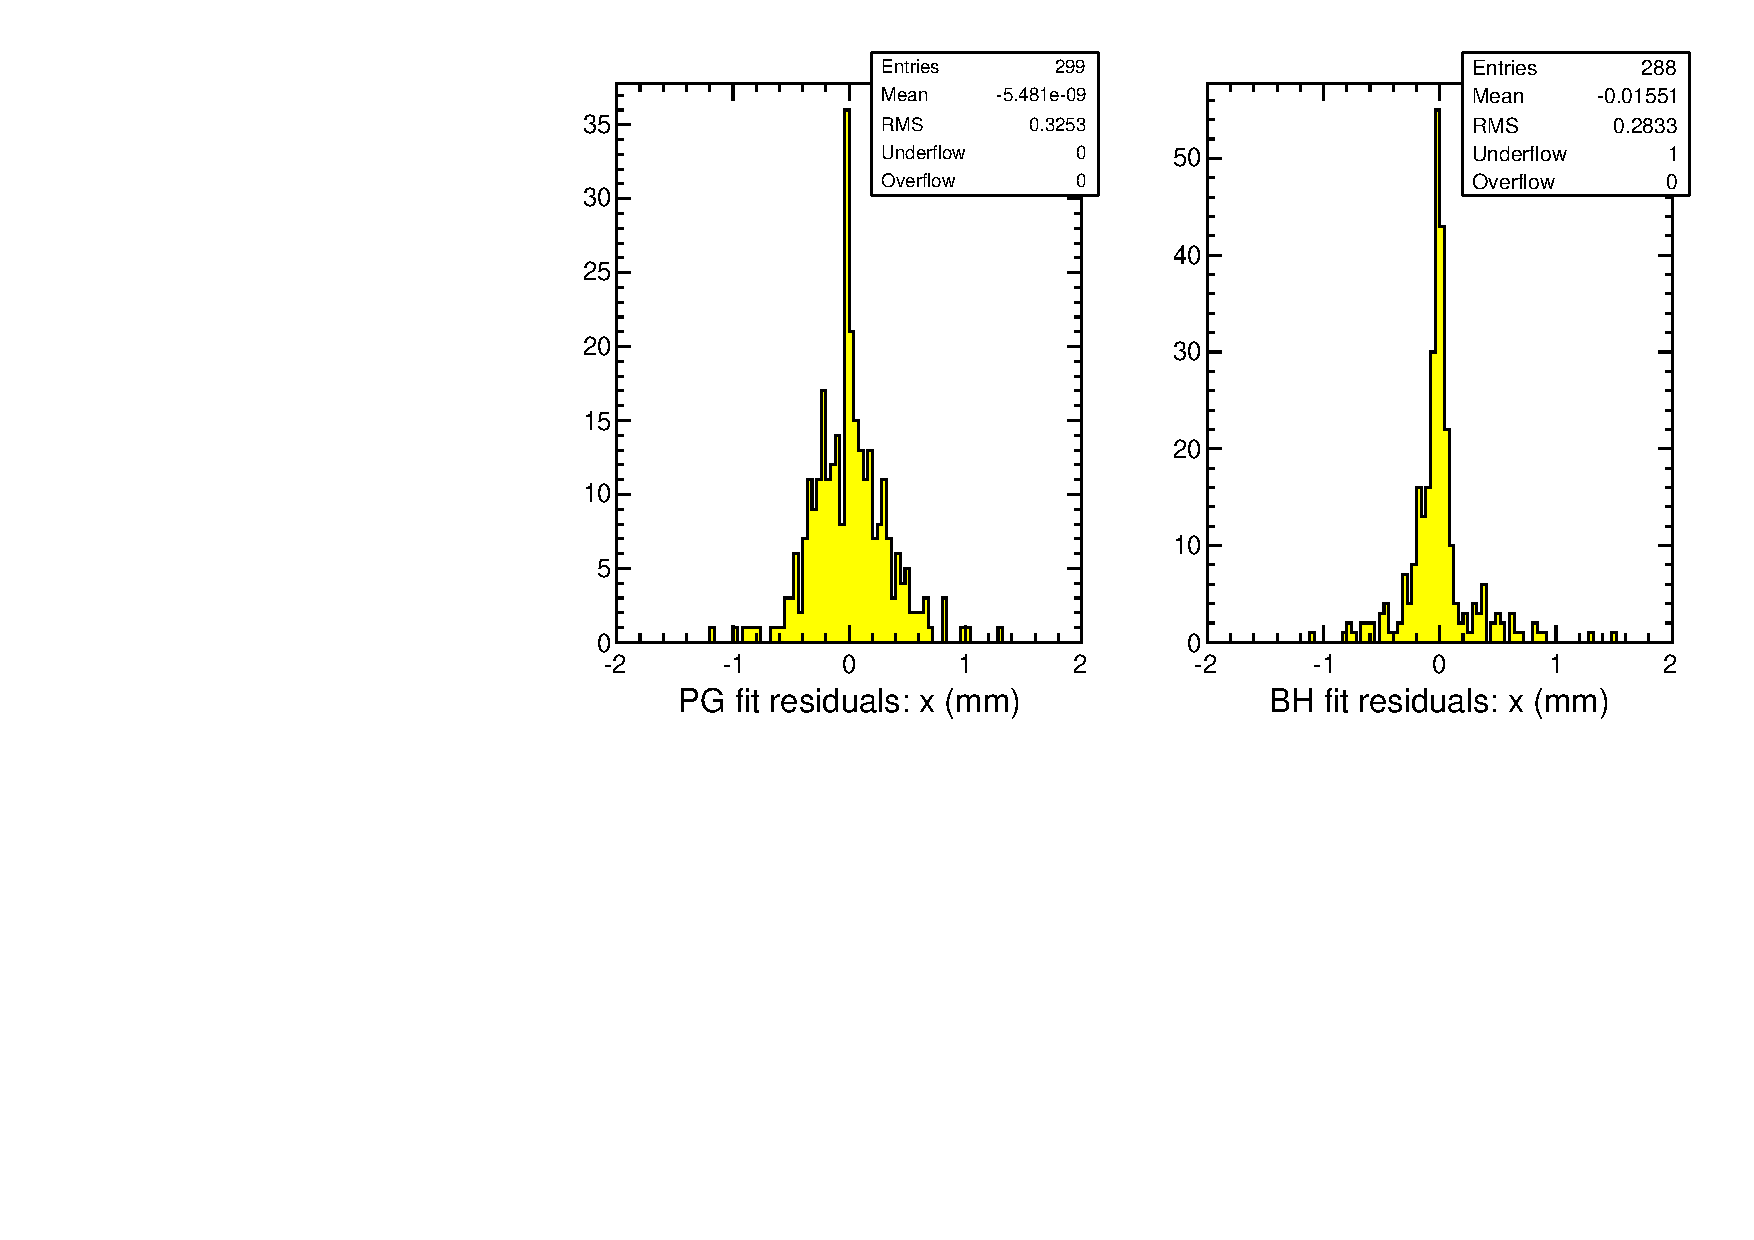
\includegraphics[width=\linewidth]{allplots_fit_residuals.pdf}

\vspace{0.5 cm}
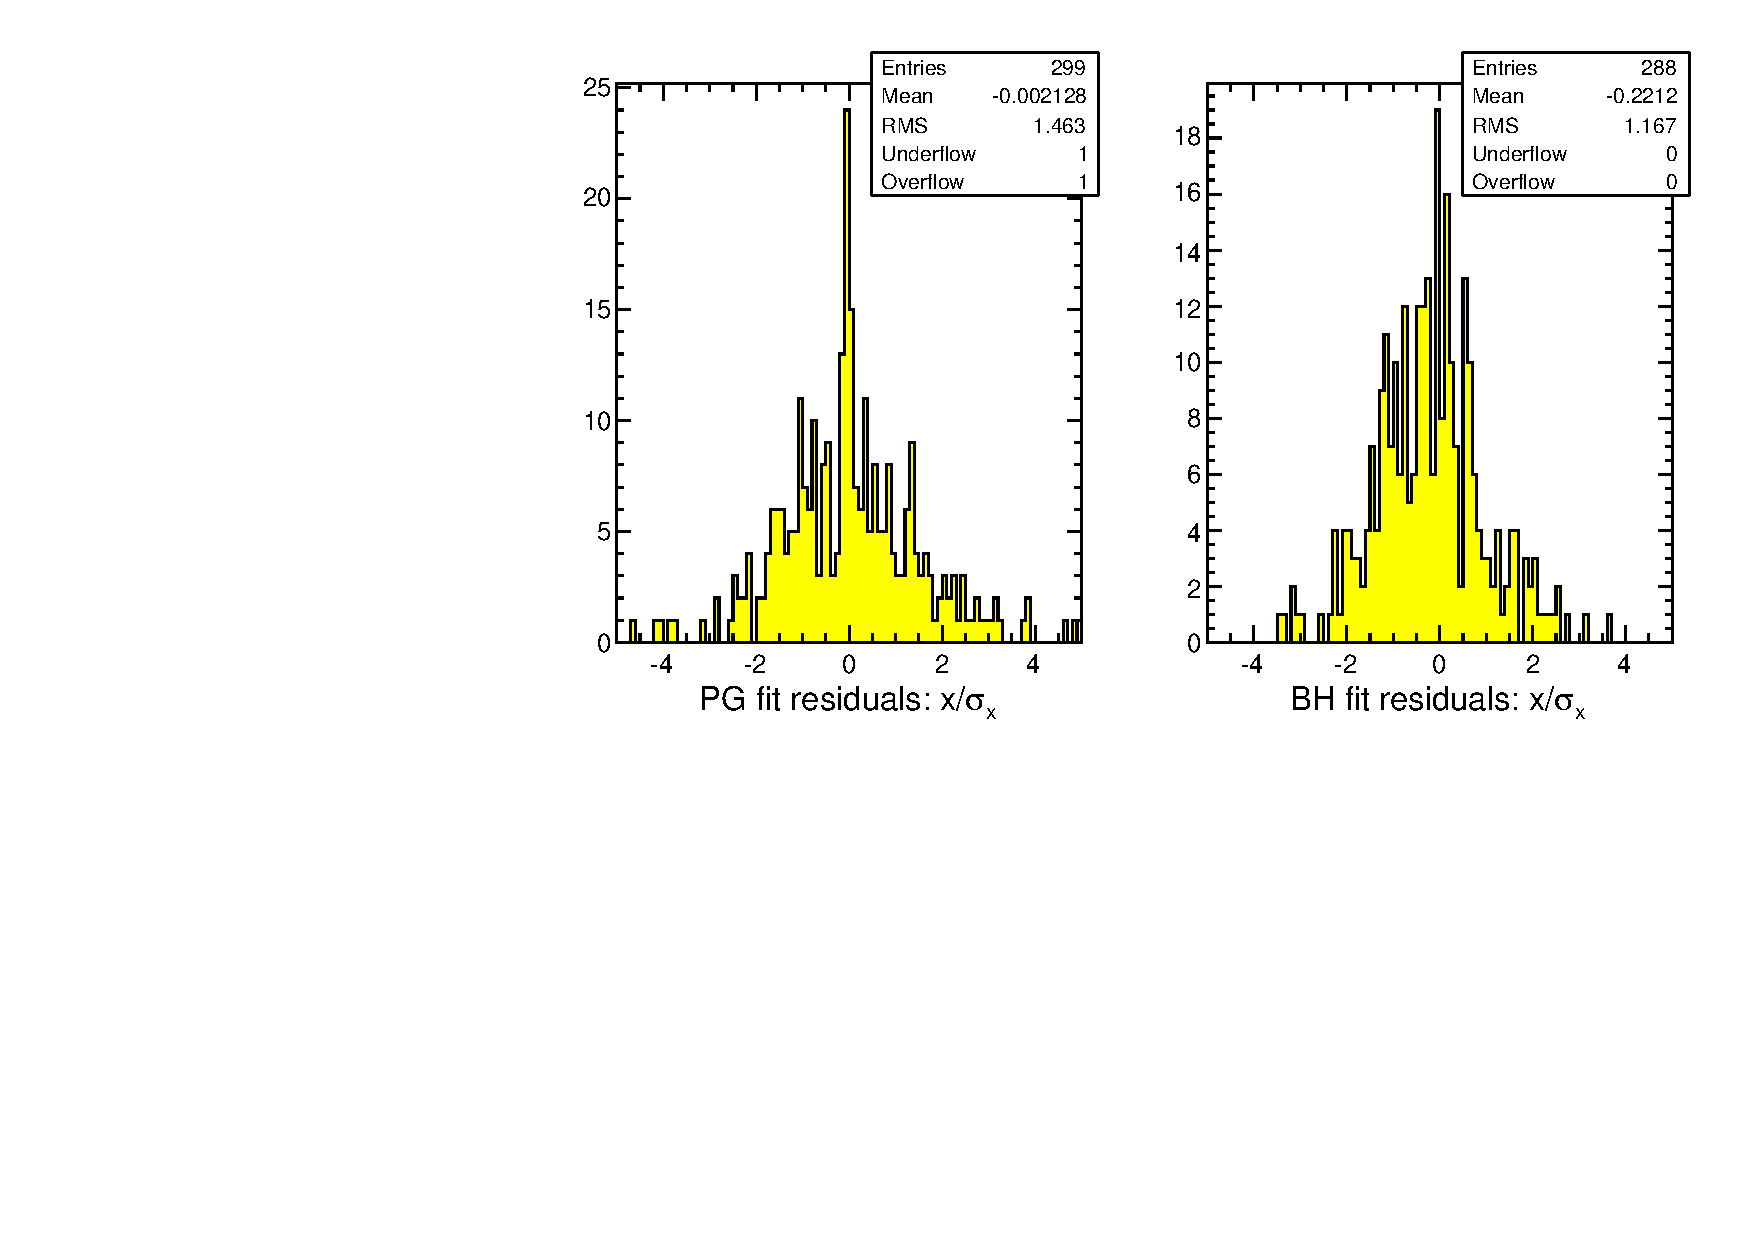
\includegraphics[width=\linewidth]{allplots_fit_residualsNorm.pdf}

\column{0.4\linewidth}
\begin{itemize}
\item Plot PG and beam-halo residuals with respect to the combined alignment solution

\item Each are compatible with the solution at the level of 0.3~mm

\item Level of statistical compatibility: $x/\sigma_x \sim 1.4$
\end{itemize}
\end{columns}
\end{frame}

\begin{frame}
\frametitle{Compatibility of PG and BH}

\begin{columns}
\column{0.6\linewidth}
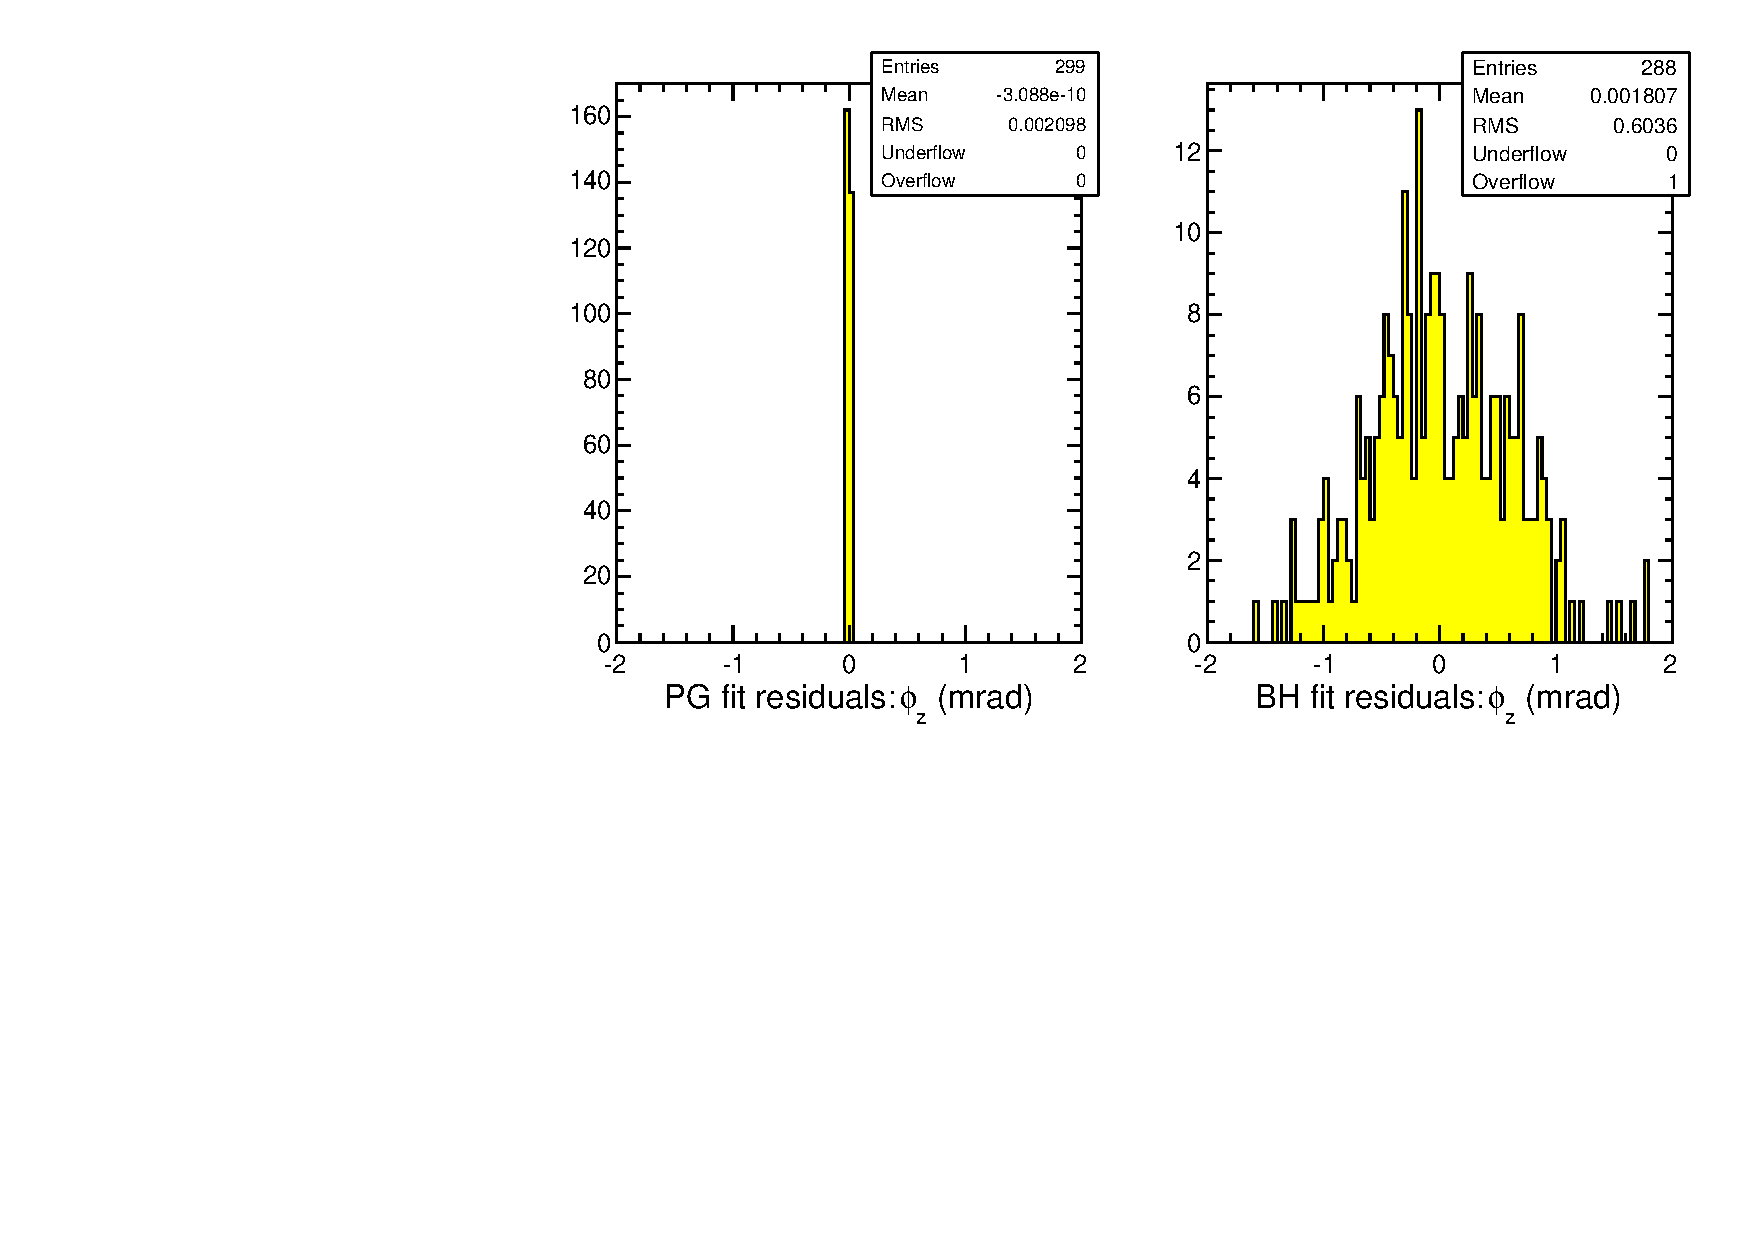
\includegraphics[width=\linewidth]{allplots_fit_angles.pdf}

\vspace{0.5 cm}
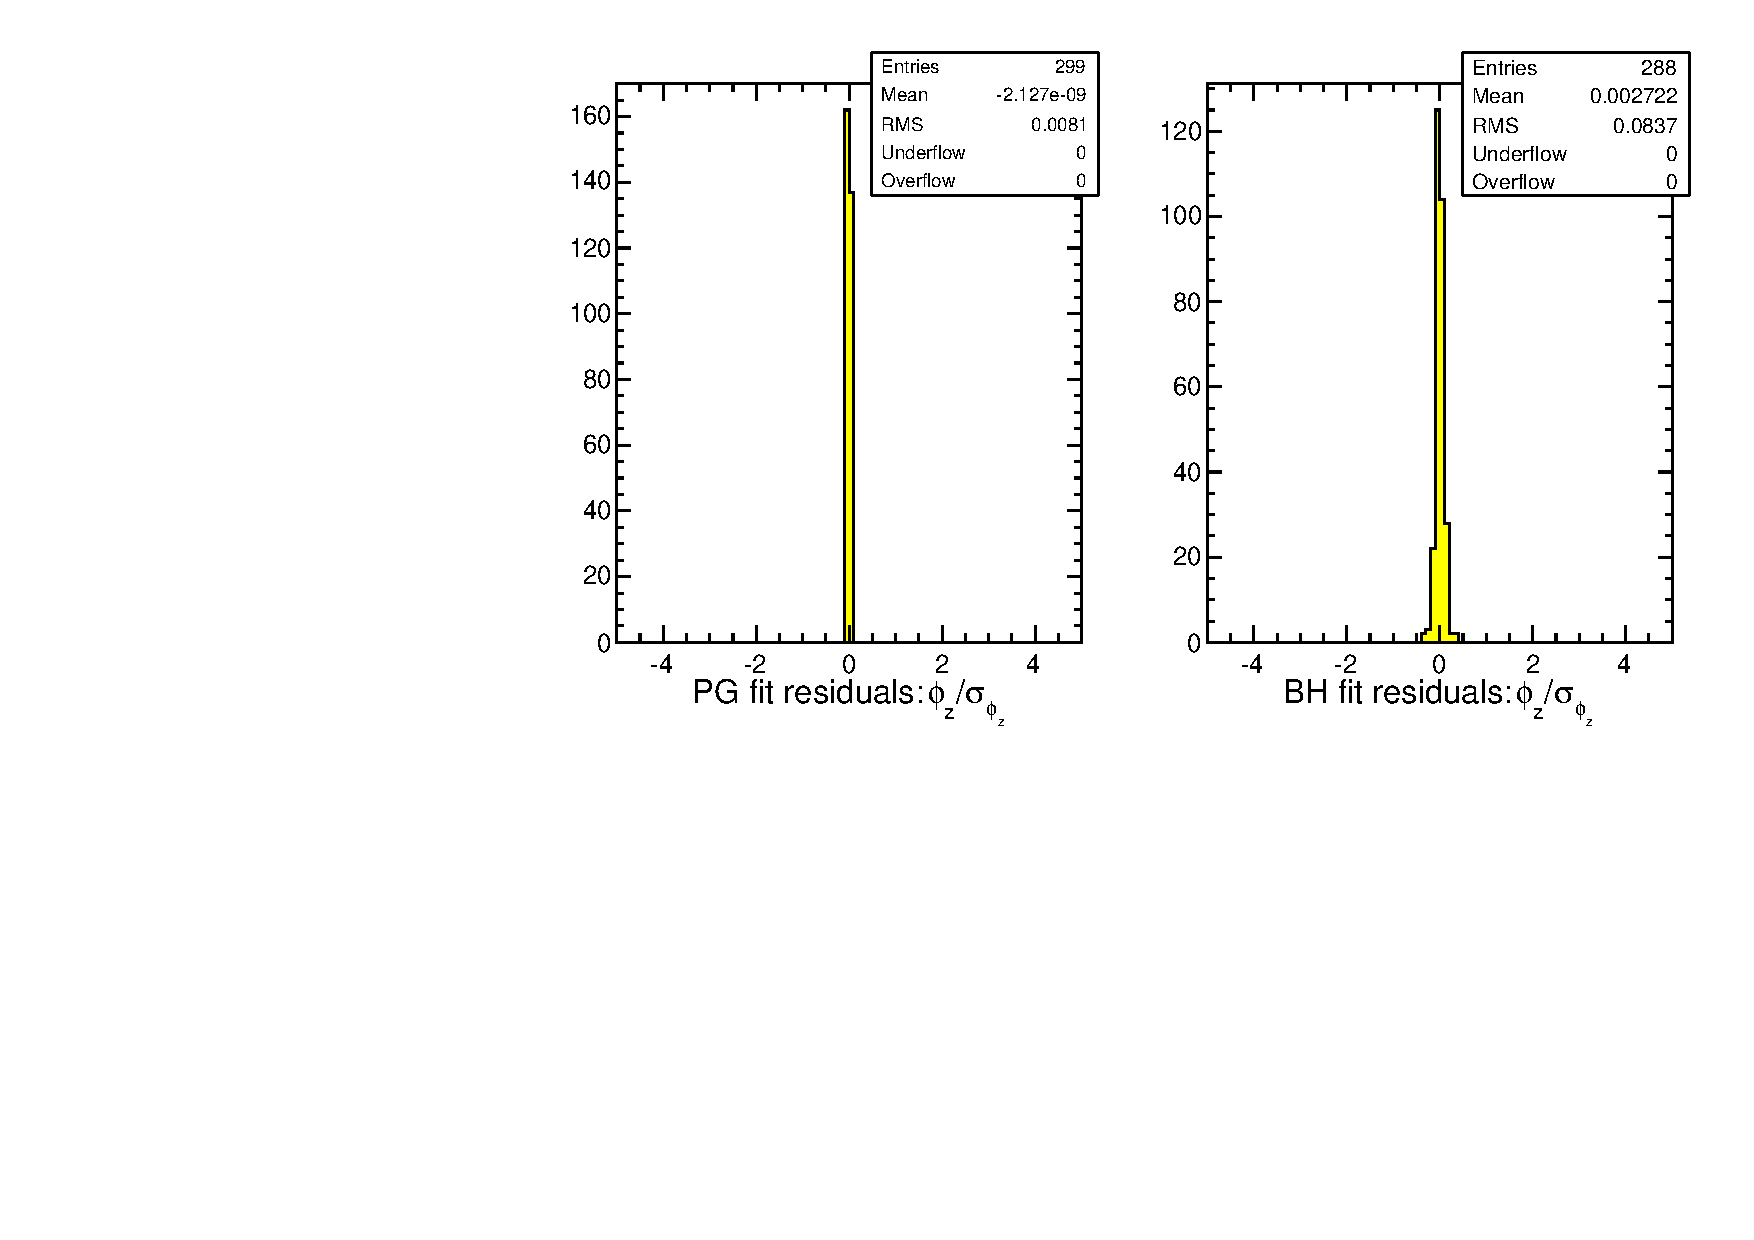
\includegraphics[width=\linewidth]{allplots_fit_anglesNorm.pdf}

\column{0.4\linewidth}
\begin{itemize}
\item Same for $\phi_z$ angles

\item Beam-halo $\phi_z$ uncertainties are overestimated, and the fit takes the PG values

\item Beam-halo $\phi_z$ agree with this on the level of 0.6~mrad; this is just a matter of weighting them properly

\item I've found the problem and am working on a solution\ldots
\end{itemize}
\end{columns}
\end{frame}

\begin{frame}
\frametitle{Error analysis ($r\phi$)}

\begin{itemize}\setlength{\itemsep}{0.25 cm}
\item What is the uncertainty in chamber positions?
\begin{itemize}
\item a complicated question because chamber uncertainties are highly
  correlated by the system of equations
\end{itemize}
\item However, the system can be decomposed into statistically
  independent modes, each of which is a linear combination of chamber
  positions, a normalized direction in $N_{\mbox{\scriptsize alignables}}$-dimensional space with an associated uncertainty.  Example mode:

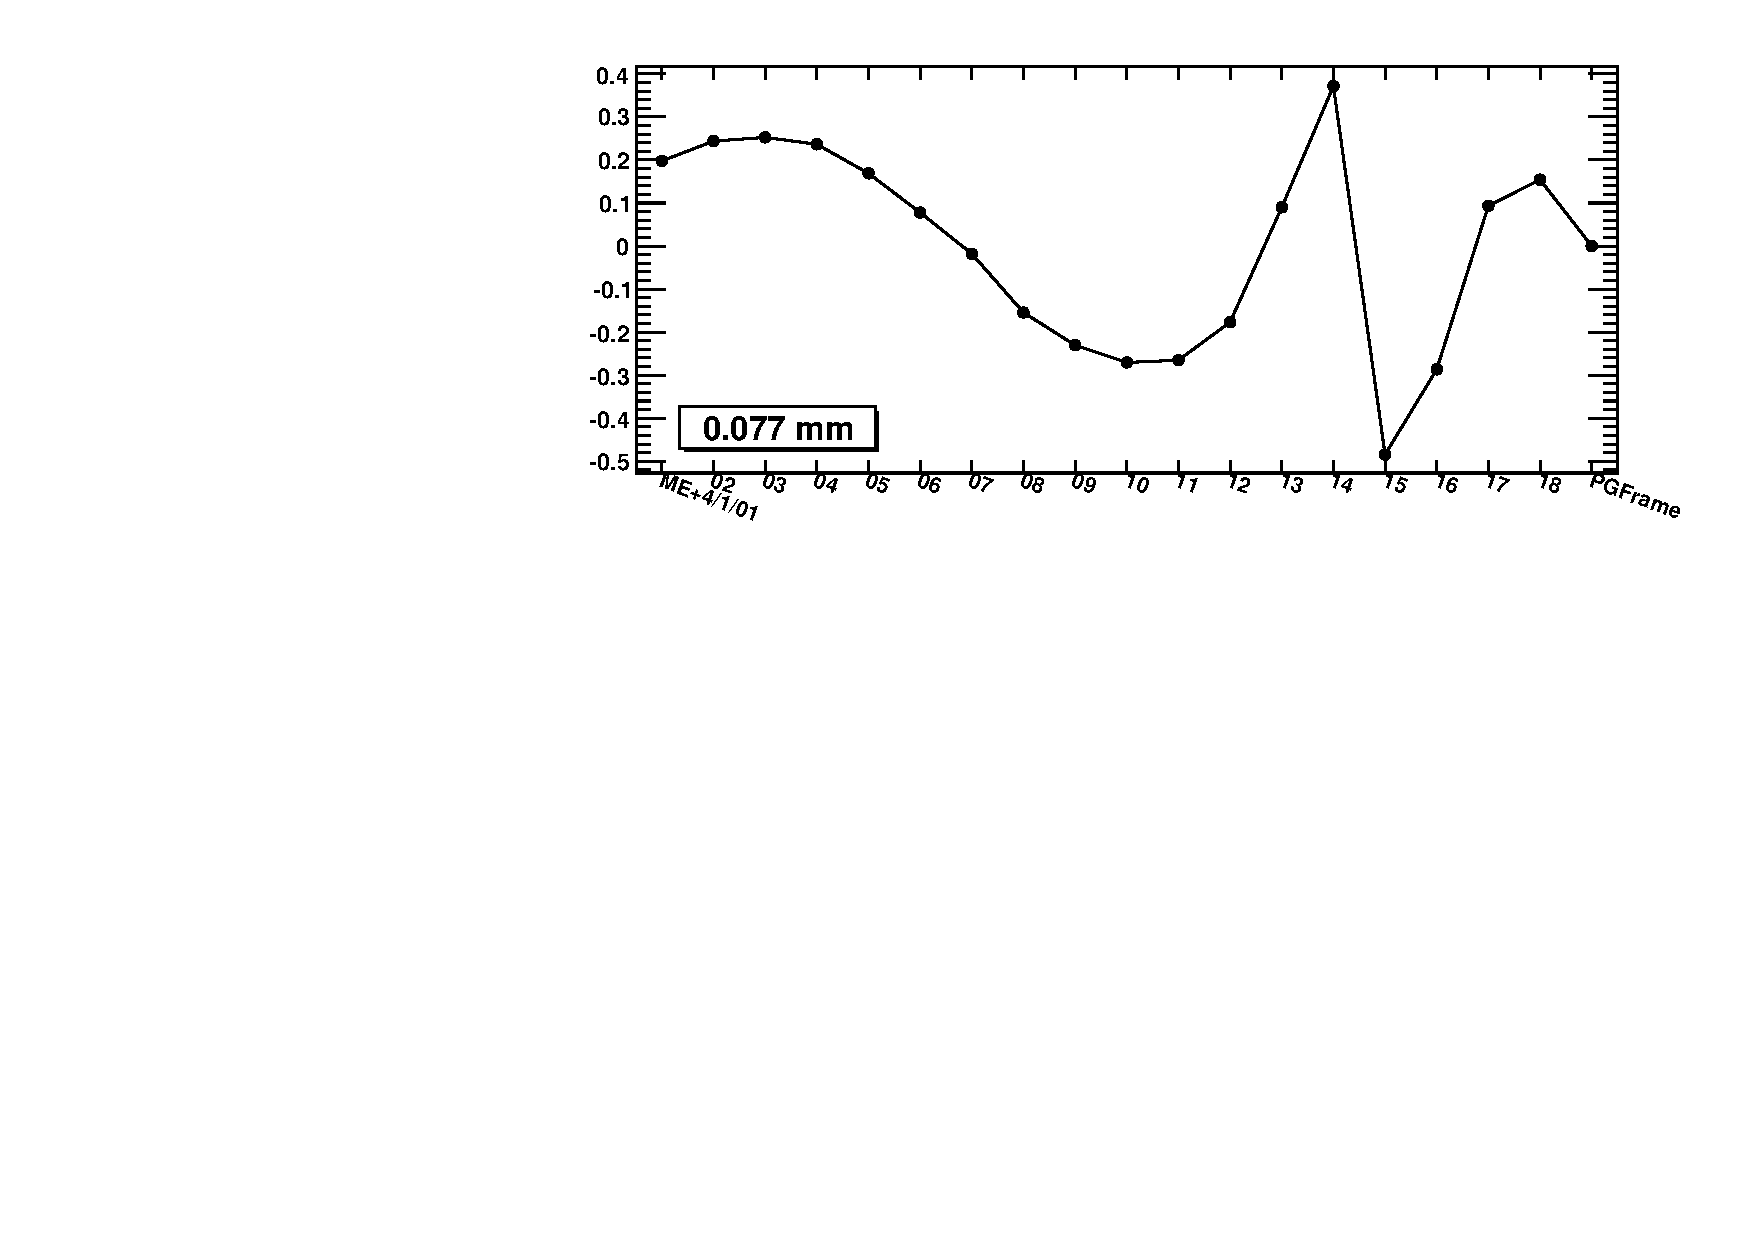
\includegraphics[width=0.8\linewidth]{example_errormode.pdf}

\item The modes with largest uncertainty are called {\it weak modes} and are generally smoother than the strong modes
\end{itemize}
\end{frame}

\begin{frame}
\frametitle{Error analysis ($r\phi$)}

\begin{itemize}
\item All modes in ME+4/1 (uncertainties in mm)

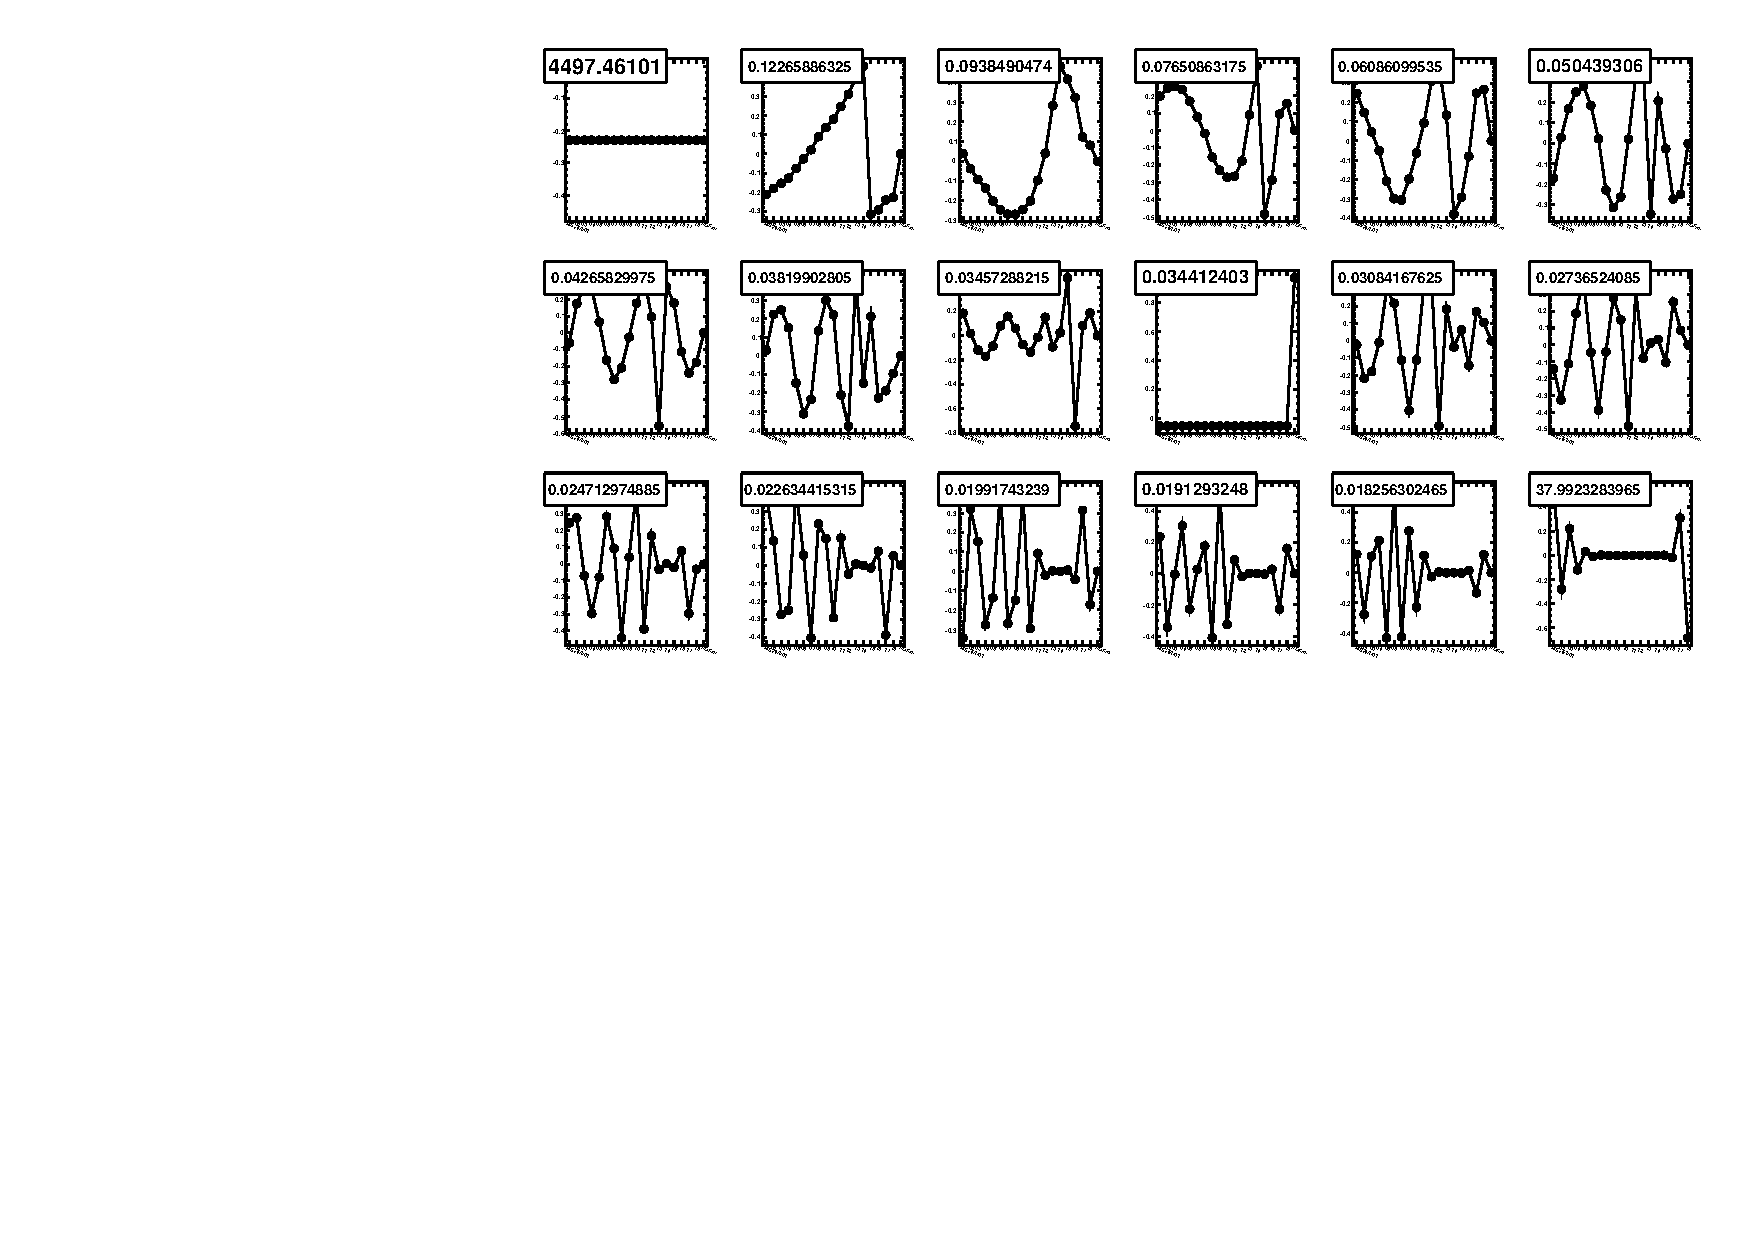
\includegraphics[width=\linewidth]{errormodes_pgnormal_p41.pdf}

\item First mode is the undetermined rigid-body position of the whole
  ring, controlled with a Lagrange multiplier (proportional to an
  arbitrary constant, set to a large number)

\item Complete set: \href{https://hypernews.cern.ch/HyperNews/CMS/get/muon-alignment/513.html}{\tt \tiny https://hypernews.cern.ch/HyperNews/CMS/get/muon-alignment/513.html}
\end{itemize}
\end{frame}

\begin{frame}
\frametitle{Error analysis}

\begin{itemize}
\item Statistical uncertainties are in the range of a few hundred microns
\end{itemize}

\renewcommand{\arraystretch}{1.1}

\begin{center}\begin{tabular}{c c c}
\hline\hline
ring & largest mode (mm) & sum in quadrature of all (mm) \\\hline
ME$+$1/1 & 0.29 & 0.54 \\
ME$+$1/2 & 0.20 & 0.60 \\
ME$+$2/1 & 0.14 & 0.23 \\
ME$+$2/2 & 0.26 & 0.76 \\
ME$+$3/1 & 0.11 & 0.19 \\
ME$+$3/2 & 0.24 & 0.70 \\
ME$+$4/1 & 0.12 & 0.21 \\\hline
ME$-$1/1 & 0.47 & 0.79 \\
ME$-$1/2 & 0.15 & 0.51 \\
ME$-$2/1 & 0.13 & 0.21 \\
ME$-$2/2 & 0.15 & 0.69 \\
ME$-$3/1 & 0.09 & 0.18 \\
ME$-$3/2 & 0.19 & 0.67 \\
ME$-$4/1 & 0.10 & 0.18 \\\hline\hline
\end{tabular}\end{center}
\end{frame}

\begin{frame}
\frametitle{Ring alignment with 2010 data}

\begin{itemize}
\item Now performed in an automated way (new script by Vadim)
\item Preliminary plot: seems to be working

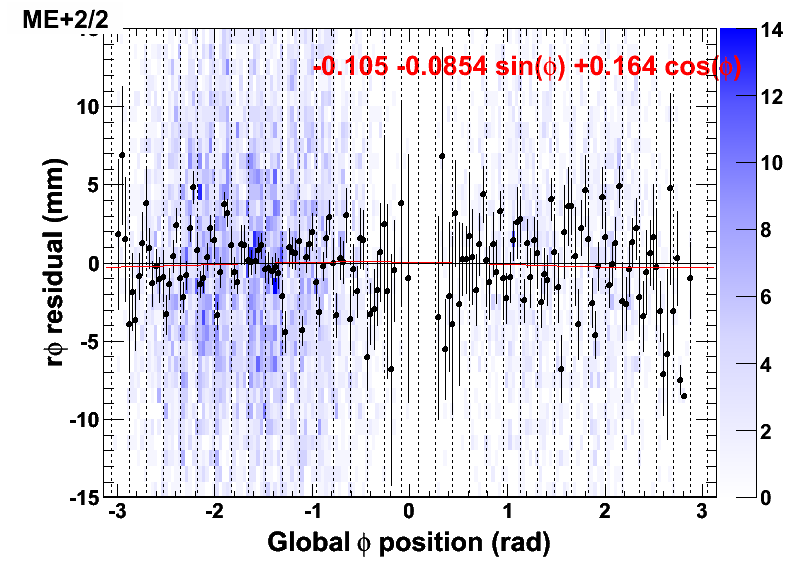
\includegraphics[width=0.7\linewidth]{map_CSCvsphi_x.png}

\item Lower efficiency on the top of CMS ($\phi > 0$) than bottom:
  more like CRAFT-08 than CRAFT-09
\item Low statistics is an issue for some rings (especially ME$x$/1)
\end{itemize}
\end{frame}

\begin{frame}
\frametitle{Conclusions}

\begin{itemize}
\item For now, using track closure as a measurement of ring-radii
\begin{itemize}
\item assumes CSC widths are well known, and we have $\vec{B}=0$ data validating that
\end{itemize}
\item Produced a complete set of CSC beam-halo constants, regardless
  of completeness of rings
\begin{itemize}
\item ME1/1: without PG constraints--- missing data lead to piecewise lack-of-constraint
\item all others except ME1/3: aligned {\it with} PG constraints--- formed a mutually consistent solution
\item ME1/3: no overlaps--- only PG
\end{itemize}

\item Final constants for next Monday or earlier

\item Final sign-off next Wednesday
\end{itemize}

\label{numpages}
\end{frame}

\begin{frame}
\frametitle{Mathematical framework}

\begin{columns}
\column{0.5\linewidth}
\vspace{0.5 cm}
\only<1>{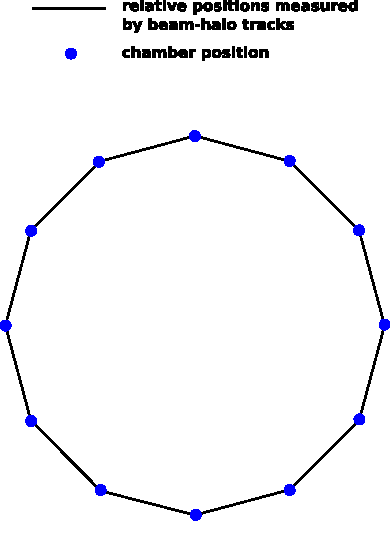
\includegraphics[width=\linewidth]{beamhalo0.pdf}}
\only<2>{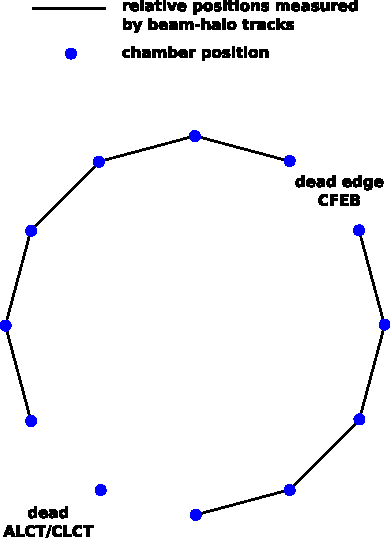
\includegraphics[width=\linewidth]{beamhalo.pdf}}
\only<3>{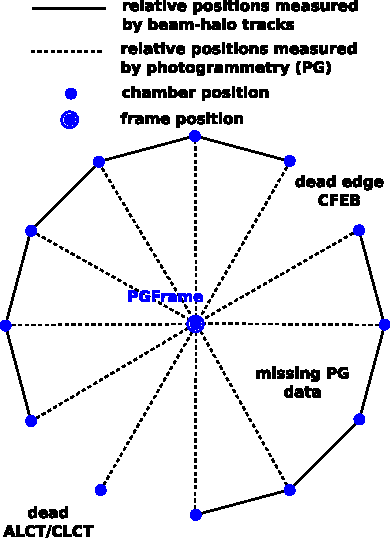
\includegraphics[width=\linewidth]{beamhalo-PG.pdf}}
\only<4>{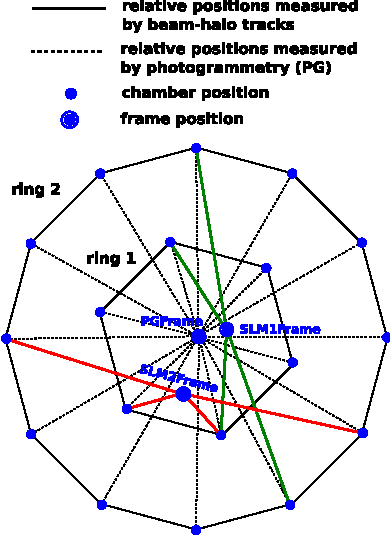
\includegraphics[width=\linewidth]{beamhalo-PG-SLM.pdf}}

\column{0.5\linewidth}
\only<1>{\begin{itemize}
\item Residuals relate chambers $i$ and $i+1$: for $N$ chambers,
  that's $N$ equations
\item Rotation angle of whole ring cannot be determined, so really only
  $N-1$ independent equations
\item Last constraint is closure:

\mbox{ } \hfill $\displaystyle \frac{1}{N}\sum_{i}^{N} r_i$ should be zero \hfill \mbox{ }
\end{itemize}}
\only<2>{\begin{itemize}
\item If one constraint is missing, we could fill in the information
  by {\it assuming} closure

\item Problem: closure became non-zero when the field was turned on
  (will revisit later in this talk)

\item Another problem: many rings had more than one missing
  constraint--- system is underdetermined

\item However, in complete rings we find that photogrammetry (PG) is still
  accurate: can use PG as a new constraint
\end{itemize}}
\only<3-4>{\begin{itemize}
\item New framework to combine beam-halo and PG on an
  equal footing:
\begin{itemize}
\item generalize equations to relate any $i$ and $j$
\item PG measurements relate each chamber $i$ with an external frame,
  a new chamber-like object
\end{itemize}
\item Even with gaps in beam-halo and PG, the system is always
  constrained or overconstrained (graph is fully connected)
\item<4> Potential extension (not in this talk): SLMs also relate
  groups of chambers to frames; I made new software flexible enough to
  possibly include it
\end{itemize}}
\end{columns}
\end{frame}

\begin{frame}
\frametitle{Ring alignment with 2010 data}

\begin{itemize}
\item We once had issues with low-momentum cosmics: do we still?
\item This is all preliminary--- literally a first look
\end{itemize}

\begin{columns}
\column{0.5\linewidth}

CRAFT-09 and -10 \\ {\scriptsize ($p_T > 40$~GeV, relative to ideal)}

\vspace{0.2 cm}
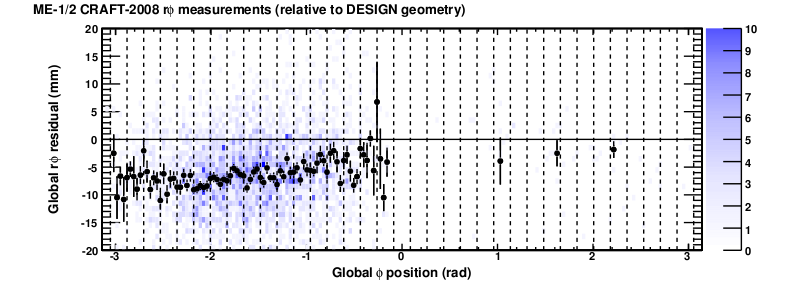
\includegraphics[width=\linewidth]{alternation_2008_mem12_design.png}

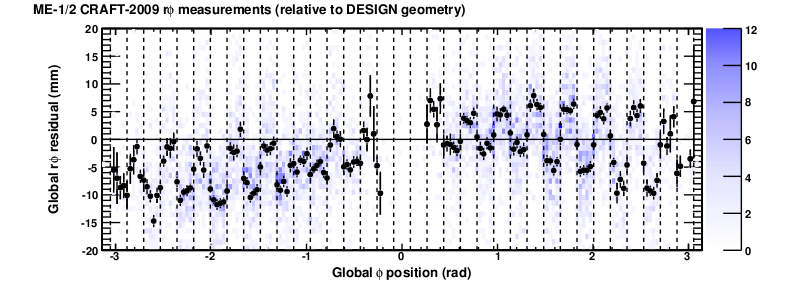
\includegraphics[width=\linewidth]{alternation_2009_mem12_design.png}

\column{0.5\linewidth}

2010 cosmic rays \\ {\scriptsize ($20 < p_T < 100$~GeV, relative to -09)}

\vspace{0.2 cm}
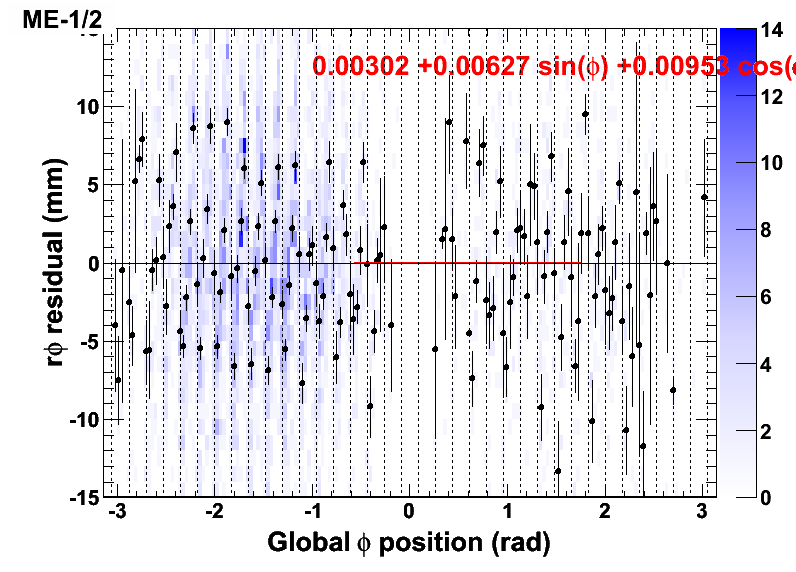
\includegraphics[width=\linewidth]{sawtooth.png}

\end{columns}

\begin{itemize}
\item The even-vs-odd alternation (which was never understood) is gone
\item It has been replaced by a residual-vs-$\phi$ slope in each chamber
\begin{itemize}
\item this effect is also seen in the barrel (``sawtooth effect'')
\end{itemize}
\end{itemize}
\end{frame}

\end{document}
